% !TEX TS-program = LuaLaTeX

\documentclass[12pt]{article}

\usepackage[urw-garamond]{mathdesign}
\usepackage[T1]{fontenc}
\usepackage{fontawesome}
\usepackage{enumitem}
\usepackage{scrextend}
\usepackage{etaremune}
\usepackage[rightcaption]{sidecap}
 
\usepackage{graphicx} %package to manage images 

% use http link for email
\usepackage[colorlinks = true,
          linkcolor = MidnightBlue,
           urlcolor  = MidnightBlue,
           citecolor = MidnightBlue,
           anchorcolor = MidnightBlue]{hyperref}            
            
%allow formula formatting
\usepackage{amsmath}
\DeclareMathAlphabet\mathbfcal{OMS}{cmsy}{b}{n}
\usepackage{comment}

%title positon
\usepackage{titling} %fix title
\setlength{\droptitle}{-6em}   % Move up the title 

%change section title font size
\usepackage{titlesec}
\titleformat{\section}
  {\normalfont\fontsize{12}{15}}{\thesection}{1em}{}[{\titlerule[0.5pt]}]
  
\titleformat{\subsection}
  {\normalfont\fontsize{12}{13}}{\thesection}{1em}{}

% change page margin and cancel identation
\usepackage[top=0.8in, bottom=0.8in, left=0.7in, right=0.7in]{geometry} 
\setlength{\parindent}{0pt}

%allow modifying section titles 
\usepackage[dvipsnames]{xcolor}

% Make lists without bullets
\renewenvironment{itemize}{
  \begin{list}{}{
    \setlength{\leftmargin}{1.5em}
    \setlength{\itemsep}{0in}
  }
}{
  \end{list}
}


\begin{document}

    \begin{flushleft}
    \textbf{
    {\huge C}{\Large HROM} {\huge N}{\Large ET--Chromatin-based cellular phenotype classification}}\\
     \hspace*{4mm} Caleb Lareau, BST 290 Midterm\\
     \hspace*{4mm} Prepared for 5 November 2016
         \end{flushleft}

%\begin{addmargin}[6.5mm]{4mm}   
\section{\textbf{{\Large A}{\small BSTRACT }}}
Recent advances in stem cell technology have enabled the isolation of induced pluripotent stem cells from committed cell lineages, providing a powerful framework for novel therapeutics and investigating cell-fate decisions. To assess factors relevant to inducing pluripotency, bioinformatics approaches have been proposed using transcriptional regulatory networks with some success. However, as transcriptional data can fail to clearly distinguish cellular phenotypes, we hypothesized that these methodological advancements could be improved. Thus, we introduce ChromNet, a novel computational approach that assigns cellular phenotypes to new samples using a reference panel of chromatin accessibility from ATAC-Seq data. We apply ChromNet to induced pluripotent cell states from blood and identify novel transcription factors associated with development cascades and cell-fate decision. 

 \section{\textbf{{\Large I}{\small NTRODUCTION}}}
The discovery of induced pluripotent stem cells (iPSC) from committed cell lineages has revolutionized cell biology.\textsuperscript{1} In particular, the ability to induce pluripotent cell states from committed lineages has afforded a remarkable experimental program to discern 

\begin{SCfigure}[0.5][h]
\caption{Growth of ATAC-Seq. Since the original description of the protocol in 2013, more than 2,000 samples are publicly available on GEO in both mouse and human. Additionally, the growth of this assay is increasing exponentially. New assays added each year are noted in the bar graphs stratified by organism. These numbers only consider bulk samples that could be downloaded from GEO determined by HTML scrubbing, but additional samples may be available through other public resources and in single cells. }
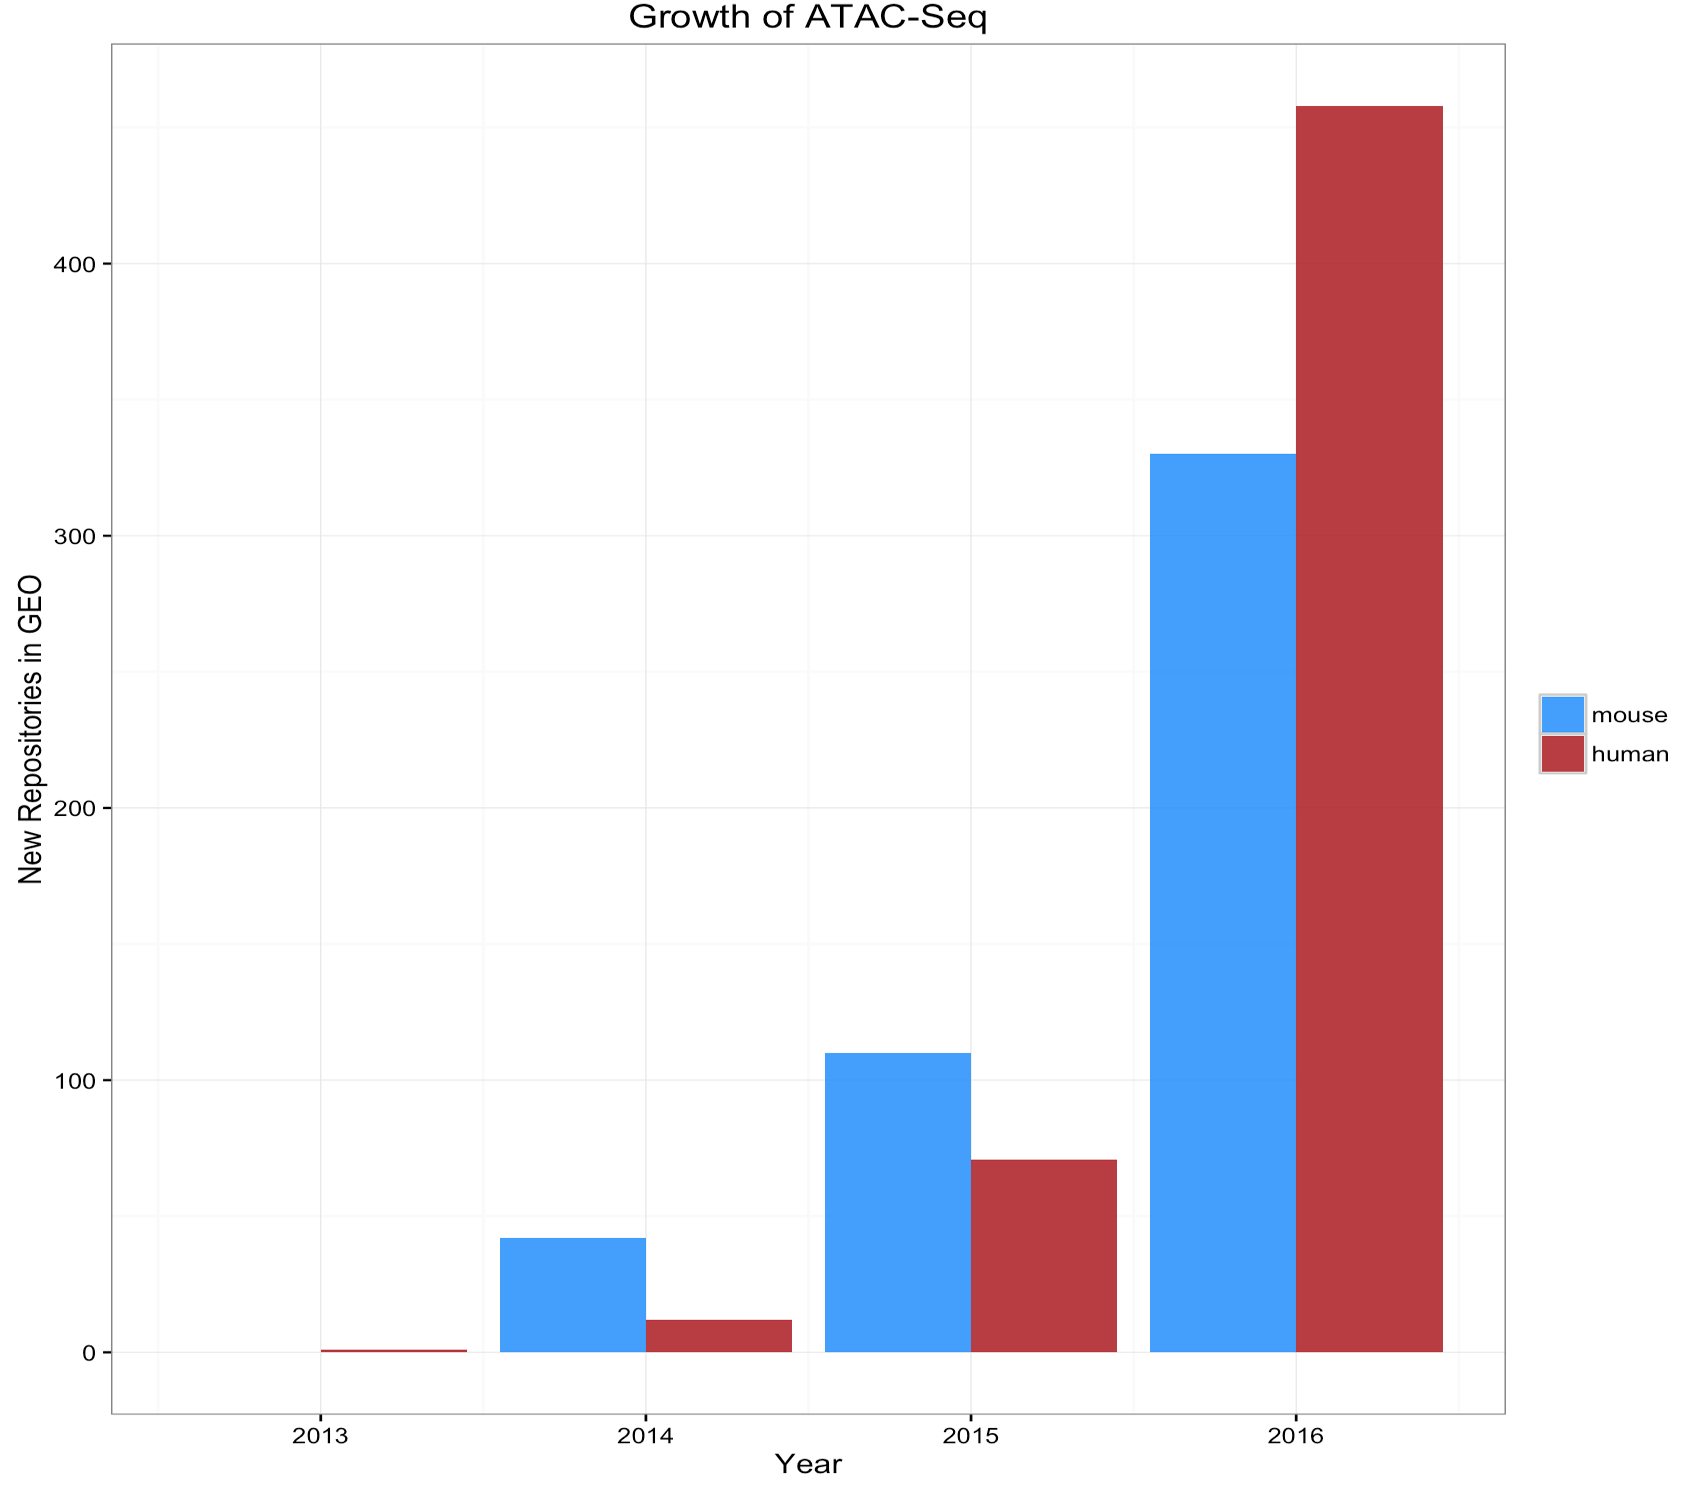
\includegraphics[scale=0.45]{atac_growth.png}
\end{SCfigure}

\begin{table}[h]
\begin{center}
  \begin{tabular}{ | c | c | c | c | c | }
    \hline
    \multicolumn{5}{ |c| }{Cluster purities of hematopoietic cells} \\ \hline
    Data Type & RNA-Seq & ATAC-Seq & Promoter ATAC & Distal Enhancer ATAC\\ \hline
    Cluster Purity & 0.776 & 0.857 & 0.675 & 0.909 \\ \hline 
  \end{tabular}
  \caption{Cluster purities of hematopoietic cells from a previous manuscript.\textsuperscript{4} While these cellular phenotypes are closely related, variable open chromatin at distal enhancer regions enables a strong separation of these phenotypes in the samples considered. Transcriptomic data as well as open chromatin at promoters were less effective in distinguishing cellular phenotypes in unsupervised clustering. }
\end{center}
\end{table}

ID factors. 

\begin{center}
\begin{figure}[h]
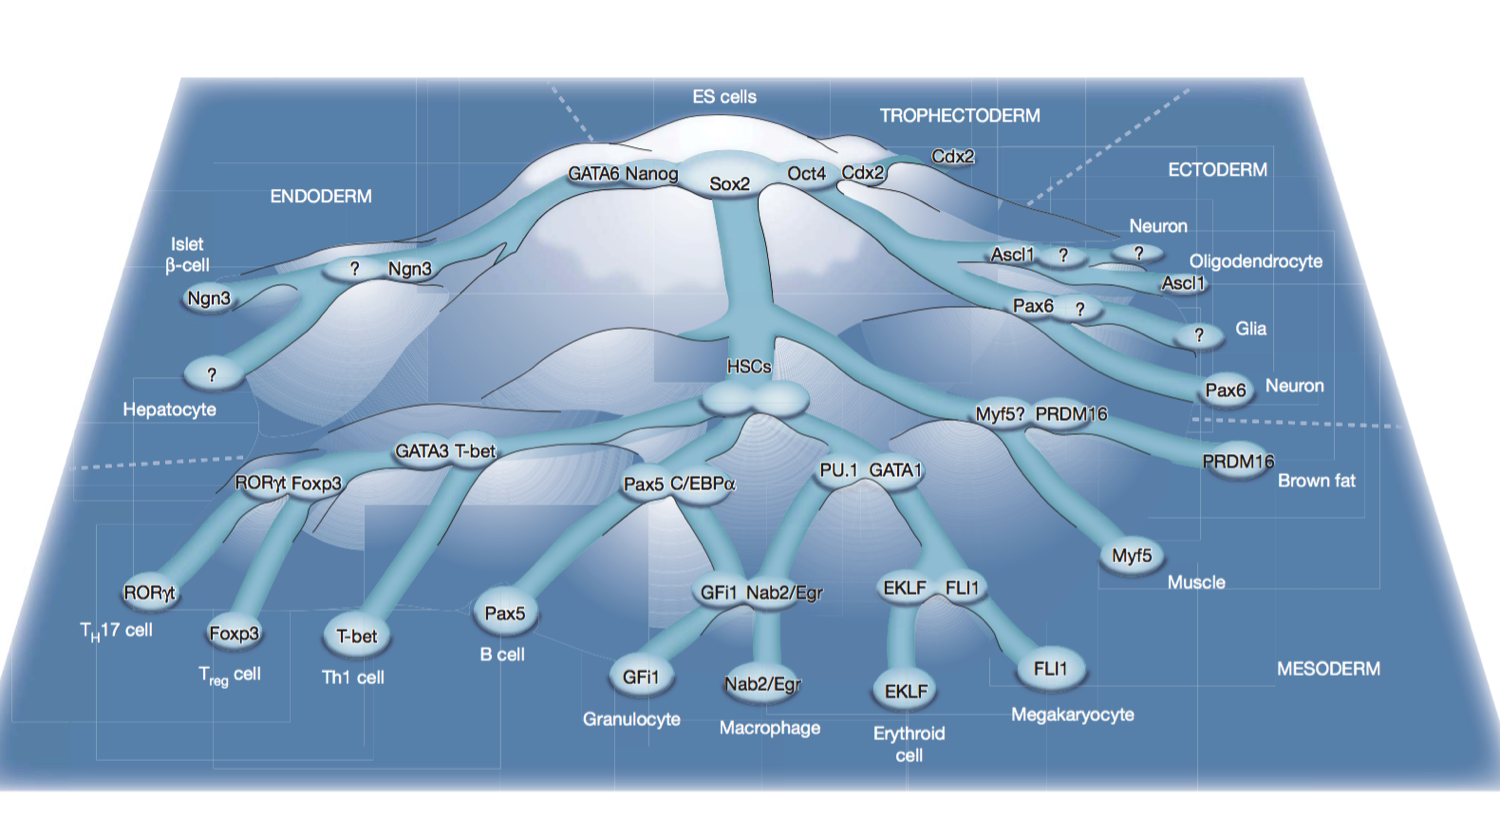
\includegraphics[width=0.85\paperwidth]{tf_landscape.png}
\caption{Transcription factors in a cascading landscape of cell states. Differentiated cell types are represented as basins whereas unstable theoretical cell states correspond to ridges and slopes in the landscape. The latter types of cells are observed infrequently during development and thus unlikely to correspond to observable cell types. Characterizing this landscape and the factors associated in moving from one type to another is vital for characterizing epigenetic plasticity. Image reproduced from a previous manuscript.\textsuperscript{5}}
\end{figure}
\end{center}

 \section{\textbf{{\Large M}{\small ETHODS}}}
 (brief)
 
 First, 
 
 To assess the efficacy of our proposed framework, 

 \section{\textbf{{\Large R}{\small ESULTS}}}
(brief) Data analysis results

(brief) Validation results

 \section{\textbf{{\Large D}{\small ISCUSSION}}}
(brief) Interpretation: 

(brief) 
 \section{\textbf{{\Large R}{\small EFERENCES}}}
 \textsuperscript{1} Yu, Junying, et al. "Induced pluripotent stem cell lines derived from human somatic cells." Science 318.5858 (2007): 1917-1920. \newline
 \textsuperscript{2} Cahan, Patrick, et al. "CellNet: network biology applied to stem cell engineering." Cell 158.4 (2014): 903-915. \newline 
 \textsuperscript{3} Buenrostro, Jason D., et al. "Transposition of native chromatin for fast and sensitive epigenomic profiling of open chromatin, DNA-binding proteins and nucleosome position." Nature methods 10.12 (2013): 1213-1218. \newline 
 \textsuperscript{4} Corces, M. Ryan, et al. "Lineage-specific and single-cell chromatin accessibility charts human hematopoiesis and leukemia evolution." Nature Genetics (2016). \newline 
 \textsuperscript{5} Graf, Thomas, and Tariq Enver. "Forcing cells to change lineages." Nature 462.7273 (2009): 587-594. \newline
%\end{addmargin}
\end{document}

